\newpage
\null
\thispagestyle{empty}
\newpage
\pagestyle{plain}
\pagenumbering{roman}
%\renewcommand{\thepage}{\Alph{page}}

%TODO dat do pice
\section{Plán ďalšej práce}

Plán a rozdelenie práce na skúškové obdobie a ďalší semester:

\begin{itemize}
	\item refaktorizácia a upratanie doterajšej práce (kód, dokumentácia)
	\item experimentácia s neurónovou sieťou - autoenkóderom
	\item postupné dodávanie ďalších informácií o scéne sieti - pre začiatok poloha objektov
	\item pripravenie experimentu pre získanie dát pre pozornosť zhora nadol (top-down)
	\item vykonanie experimentu s čo najväčším počtom ľudí
	\item vyhodnotenie
	\item otestovanie ďalších faktorov pozornosti zhora nadol
	\item experimentovanie
	\item refactor kódu
	\item porovnanie výsledkov s inými riešeniami
	\item predbežné doplnenie dokumentácie
\end{itemize}

V závislosti od problémov a dosiahnutých výsledkov počas semestra sa bude plán predbežne meniť a upravovať.

\newpage
\pagestyle{plain}
\pagenumbering{roman}
%\renewcommand{\thepage}{\Alph{page}}

%TODO upravit - pridat dataset, ulozene modely, atd. 
\section{Obsah priloženého elektronického nosiča}

Štruktúra dát na elektronickom nosiči:

\begin{itemize}
	\item \textbf{dataset} - vzorka upraveného pripraveného datasetu pre neurónovú sieť
	\item \textbf{source\_codes} - zdrojové kódy
	\item \textbf{document} - pdf verzia odovzdávanej práce
\end{itemize}

%TODO zvazit pridanie casi s velkym diagramom architektury, vyriesit cislovanie
\section{Podrobný diagram architektúry s kombináciou VGG16 a autoenkóderu}
\label{vgg16_autoencoder_architecture_detailed}
\begin{figure}[H]
	\begin{center}
		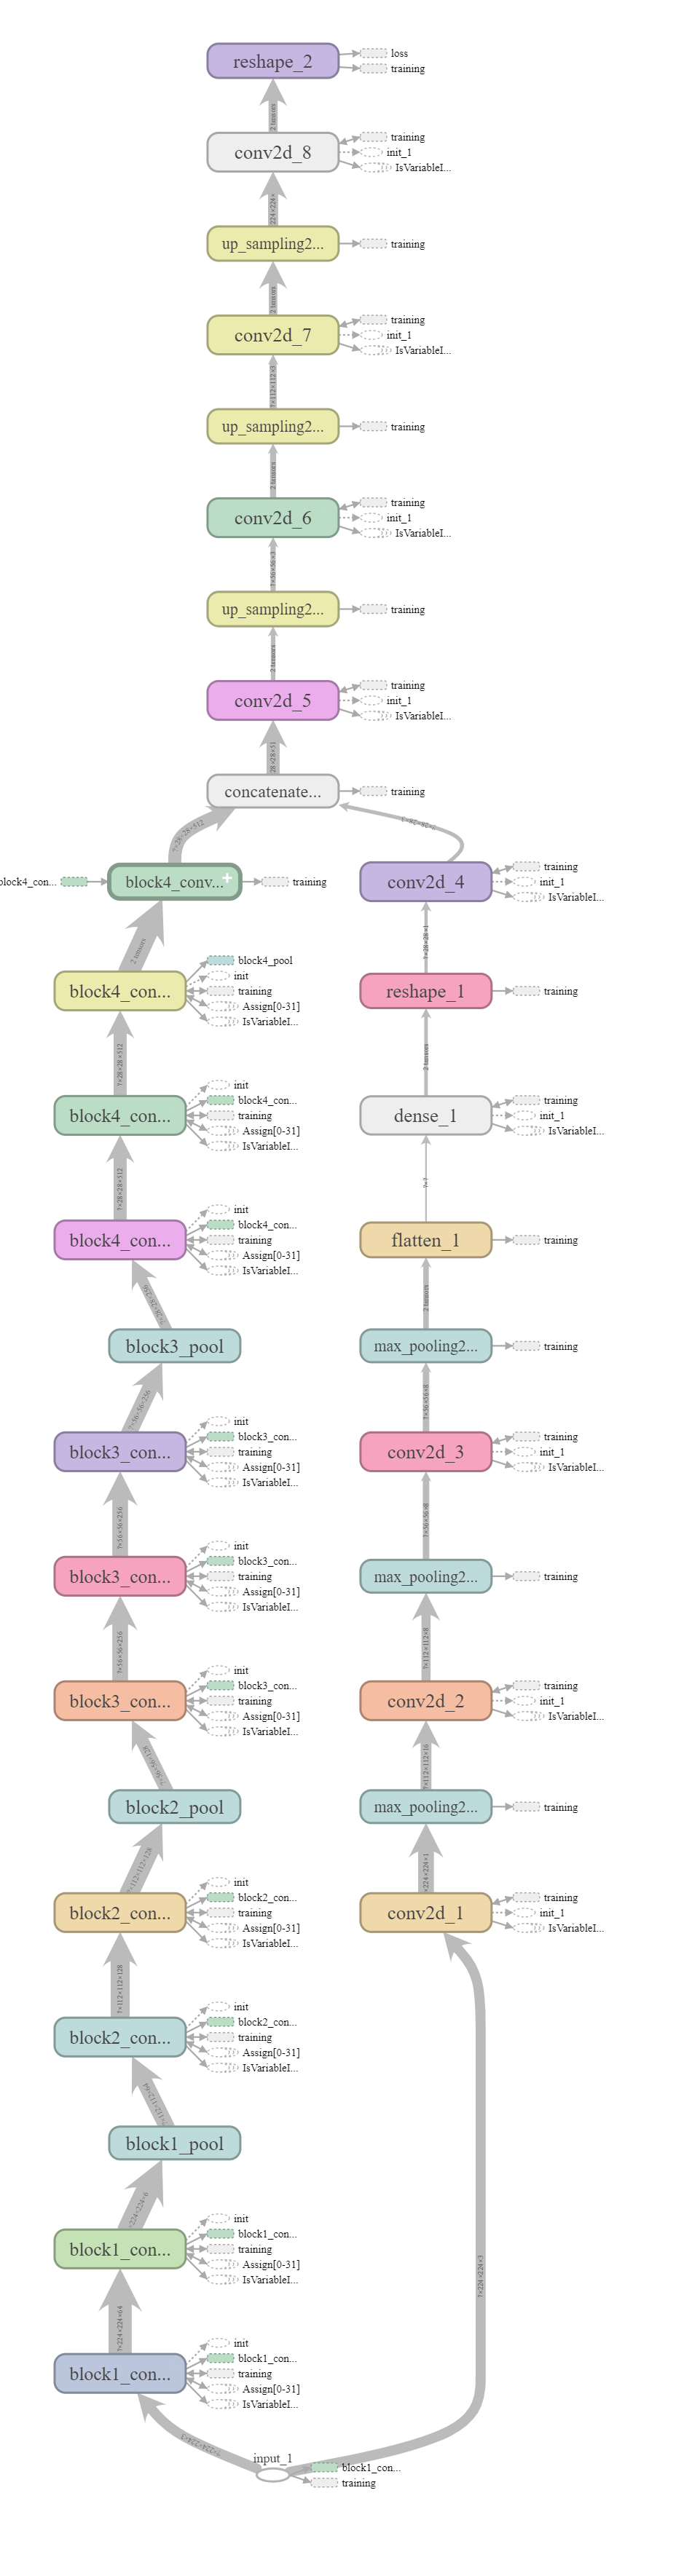
\includegraphics[scale=0.24]{vgg16_with_autoencoder_full.png}
		\caption[Podrobný diagram architektúry VGG16 s autoenkóderom]{Podrobný diagram architektúry VGG16 s autoenkóderom}
	\end{center}
\end{figure}

%TODO Technicka dokumentacia? prostredie, hardver, kniznice, atd.

%TODO pouzivatelska prirucka

%TODO plan prace na rieseni projektu? 
